\documentclass{fancyslides} 
\usepackage[utf8]{inputenc}
\usepackage{times}

\usepackage{graphicx}
\usepackage{caption}
\usepackage{subcaption}


\graphicspath{{img/}}

%%% Beamer settings (do not change)
\usetheme{default} 
\setbeamertemplate{navigation symbols}{} %no navigation symbols
\setbeamercolor{structure}{fg=\yourowntexcol} 
\setbeamercolor{normal text}{fg=\yourowntexcol} 



%%%%%%%%%%%%%%%%%%%%%%%%%
%%% CUSTOMISATIONS %%%%%%
%%%%%%%%%%%%%%%%%%%%%%%%%


%%%% SLIDE ELEMENTS
\newcommand{\structureopacity}{0.75} %opacity for the structure elements (boxes and dots)
\newcommand{\strcolor}{black} %elements colour (predefined blue; orange; green)

%%%% TEXT COLOUR
\newcommand{\yourowntexcol}{white}


%%%%%%%%%%%%%%%%%%%%%%%%%
%%% TITLE SLIDE DATA %%%%
%%%%%%%%%%%%%%%%%%%%%%%%%
\fbckg{abstract-data}
\newcommand{\titlephrase}{On-Line Analytical Processing}
\newcommand{\name}{Javier Bonet \\ Joel Catacora \\}
\newcommand{\affil}{Base de datos avanzada}
\newcommand{\email}{22 de abril del 2015}


\begin{document}


\startingslide %this generates titlepage from the data above

\fbckg{white}
\begin{frame}
\pointedsl{{\LARGE ¿Qué es OLAP?}}
\end{frame}


\fbckg{white}
\begin{frame}
\misc
{
El \textbf{procesamiento analítico en línea} (OLAP) es una solución utilizada en el campo de la inteligencia de negocios, cuyo objetivo es permitir la consulta de grandes cantidades de datos de forma eficiente y sencilla.
}
\end{frame}

\fbckg{white}
\begin{frame}
\misc
{
El concepto OLAP puede definirse mediante 5 palabras: Análisis Rápido de Información Compartida Multidimensional, (Fast Analysis of Shared Multidimensional Information, o FASMI).
}
\end{frame}

\fbckg{white}
\begin{frame}
\misc
{
\begin{itemize}
  \item \textbf{Rápida}: el sistema está dirigido a proporcionar la mayoría de las respuestas a los usuarios en pocos segundos.
  \item \textbf{Análisis}: el sistema puede hacer frente a cualquier lógica de negocio y análisis estadístico que sea relevante para el usuario, en forma relativamente sencilla.
  \item \textbf{Compartida}: significa que el sistema implementa todos los requisitos de seguridad de la confidencialidad.
  \item \textbf{Multidimensionalidad}: el sistema debe proveer una vista conceptual multidimensional de los datos.
  \item \textbf{Información}: se refiere a todos los datos y la información derivada, que sea relevante para la aplicación.
\end{itemize}
}
\end{frame}



\fbckg{white}
\begin{frame}
\pointedsl{{\LARGE Características}}
\end{frame}


\fbckg{white}
\begin{frame}
\itemized{
\item \textbf{Soportar cálculos complejos}
}
\end{frame}

\fbckg{white}
\begin{frame}
\itemized{
\item \textbf{Soportar cálculos complejos}
\item \textbf{Rapidez de respuesta}
}
\end{frame}

\fbckg{white}
\begin{frame}
\itemized{
\item \textbf{Soportar cálculos complejos}
\item \textbf{Rapidez de respuesta}
\item \textbf{Inteligencia respecto del tiempo}
}
\end{frame}


\fbckg{white}
\begin{frame}
\pointedsl{{\LARGE Reglas de Codd}}
\end{frame}

\fbckg{white}
\begin{frame}
\itemized{
\item \textbf{Visión multidimensional}
}
\end{frame}

\fbckg{white}
\begin{frame}
\itemized{
\item \textbf{Visión multidimensional}
\item \textbf{Manipulación intuitiva de los datos}
}
\end{frame}

\fbckg{white}
\begin{frame}
\itemized{
\item \textbf{Visión multidimensional}
\item \textbf{Manipulación intuitiva de los datos}
\item \textbf{Accesibilidad}
}
\end{frame}

\fbckg{white}
\begin{frame}
\itemized{
\item \textbf{Visión multidimensional}
\item \textbf{Manipulación intuitiva de los datos}
\item \textbf{Accesibilidad}
\item \textbf{Soporte multi-usuario}
}
\end{frame}

\fbckg{white}
\begin{frame}
\itemized{
\item \textbf{Visión multidimensional}
\item \textbf{Manipulación intuitiva de los datos}
\item \textbf{Accesibilidad}
\item \textbf{Soporte multi-usuario}
\item \textbf{Información separada del origen de datos}
}
\end{frame}

\fbckg{white}
\begin{frame}
\itemized{
\item \textbf{Visión multidimensional}
\item \textbf{Manipulación intuitiva de los datos}
\item \textbf{Accesibilidad}
\item \textbf{Soporte multi-usuario}
\item \textbf{Información separada del origen de datos}
\item \textbf{Flexibilidad ante valores nulos}
}
\end{frame}

\fbckg{white}
\begin{frame}
\itemized{
\item \textbf{Visión multidimensional}
\item \textbf{Manipulación intuitiva de los datos}
\item \textbf{Accesibilidad}
\item \textbf{Soporte multi-usuario}
\item \textbf{Información separada del origen de datos}
\item \textbf{Flexibilidad ante valores nulos}
\item \textbf{Rendimiento uniforme}
}
\end{frame}

\fbckg{white}
\begin{frame}
\itemized{
\item \textbf{Visión multidimensional}
\item \textbf{Manipulación intuitiva de los datos}
\item \textbf{Accesibilidad}
\item \textbf{Soporte multi-usuario}
\item \textbf{Información separada del origen de datos}
\item \textbf{Flexibilidad ante valores nulos}
\item \textbf{Rendimiento uniforme}
\item \textbf{Dimensiones y niveles de agregación ilimitados}
}
\end{frame}

\fbckg{white}
\begin{frame}
\pointedsl{\LARGE{Jerarquías}}
\end{frame}

\fbckg{white}
\begin{frame}
\misc
{
Las \textbf{jerarquías} se utilizan para especificar en menor o mayor detalle los datos contenidos en la dimensión. Las jerarquías son de mucha utilidad a la hora de calcular valores "agregados"\\ \ \\ \ \\

\underline{Ejemplos:}\\ \ \\
Dimensión tiempo $\Longrightarrow$  año-mes-día ó año-cuatrimestre-mes-día\\
Dimension producto $\Longrightarrow$ categoría-subcategoría-producto
}
\end{frame}


\fbckg{white}
\begin{frame}
\pointedsl{\LARGE{Agregaciones}}
\end{frame}

\fbckg{white}
\begin{frame}
\misc
{
Los \textbf{agregados} se utilizan en los modelos dimensionales del Data Warehouse para producir efectos positivos sobre el tiempo que toma una consulta sobre grandes conjuntos de datos. El uso más común de los agregados es tomar una dimensión y cambiar su granularidad.
Al cambiar la granularidad de la dimensión, la tabla de hechos tiene que ser parcialmente resumida para adaptarse a la nueva dimensión. Se crean así, nuevas tablas de dimensiones y tablas de hechos, que encajan en este nuevo nivel de granularidad.
}
\end{frame}

\fbckg{white}
\begin{frame}
\misc
{
\begin{figure}
        \centering
        \begin{subfigure}[b]{0.5\textwidth}
                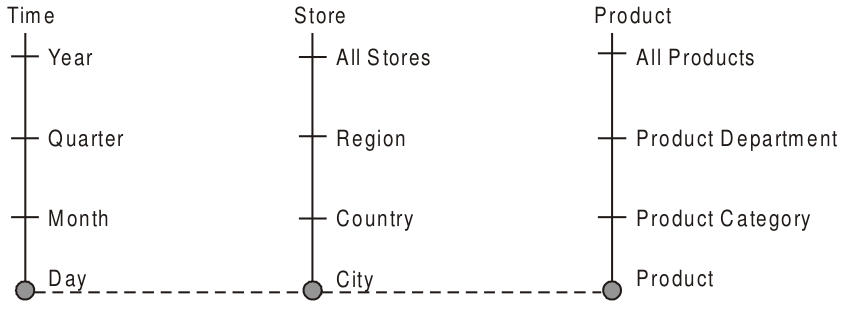
\includegraphics[width=\textwidth]{ej1_agregados}

                Esquema de nivel base que usa la parte inferior del nivel de je-rarquías dimensionales.
        \end{subfigure}%
        ~ \quad
        \begin{subfigure}[b]{0.5\textwidth}
                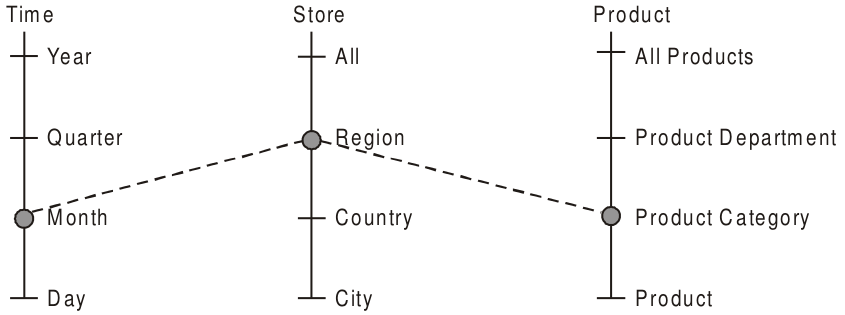
\includegraphics[width=\textwidth]{ej2_agregados}
                
                Esquema agregado, que resulta en datos de un nivel más alto en las jerarquía dimensionales.
        \end{subfigure}
\end{figure}

Los esquemas agregados proporcionan mejoras en el rendimiento debido a que tienen un número significativamente menor de registros.

}
\end{frame}


\fbckg{white}
\begin{frame}
\misc
{
\textbf{Ejemplo:}

Este esquema copo de nieve, tiene una sola tabla de echos \textit{Sales}, dos métricas (\textit{units and dollars}) y cuatro tablas de dimensiones (\textit{Product, Mfr, Customer, Time, y Customer}).

\begin{center}
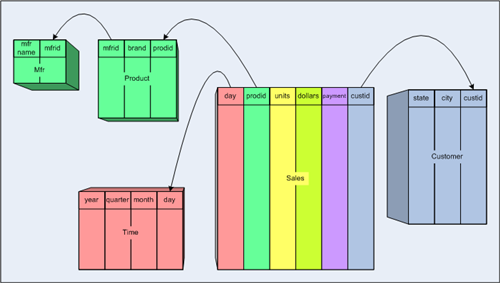
\includegraphics[scale=0.4]{aggregate_tables_1}
\end{center}
}
\end{frame}

\fbckg{white}
\begin{frame}
\misc
{
\textbf{Ejemplo:}

Creamos una tabla agregada, \textbf{Agg\_1}:
 
\begin{center}
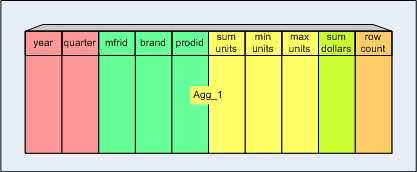
\includegraphics[scale=0.5]{aggregate_tables_2}
\end{center}
}
\end{frame}

\fbckg{white}
\begin{frame}
\misc
{Veamos como las columnas del esquema original se han combinado en la tabla \textbf{Agg\_1}:

\begin{itemize}
  \item La dimensión \textit{Time} se "colapsó" en la tabla de agregación, omitiendo las columnas \textit{month} y \textit{day}.
  \item Las dos tablas de la dimensión \textit{Product} se "colapsaron" en la tabla de agregación.
  \item La dimensión \textit{Customer} se "perdió".
  \item Para cada métrica en la tabla de hechos (\textit{units, dollars}), hay uno o más métricas en la tabla de agregación (\textit{sum units, min units, max units, sum dollars}).
  \item También hay una nueva métrica, \textit{row count}, que representa la métrica "conteo".
\end{itemize}
}
\end{frame}


\fbckg{white}
\begin{frame}
\misc
{
\textbf{Ejemplo}

Otra tabla agregada, \textbf{Agg\_2}:

\begin{center}
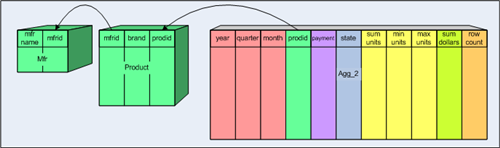
\includegraphics[scale=0.5]{aggregate_tables_3}
\end{center}

Varias dimensiones colapsaron: \textit{Time} en el nivel \textit{Quarter}; \textit{Customer} en el nivel \textit{State};
y \textit{Payment Method} a nivel \textit{Payment Method}. Pero la dimensión \textit{Product} se conservó.}
\end{frame}


\fbckg{white}
\begin{frame}
\misc
{
Tener datos agregados en el modelo dimensional hace que el entorno sea más complejo.
Para que esta complejidad adicional sea transparente al usuario, se utiliza una funcionalidad conocida como \textit{navegación de agregados},
la cual es implementada por el motor OLAP, para consultar las tablas dimensionales y de hecho, con el nivel de granularidad correcto.
}
\end{frame}

\fbckg{white}
\begin{frame}
\pointedsl{\LARGE{Hipercubo de datos}}
\end{frame}

\fbckg{white}
\begin{frame}
\misc
{
El cubo OLAP puede ser pensado como una extensión de la matriz multidimensional de una hoja de cálculo, de ahí el nombre del hipercubo. Técnicamente, el cubo de datos es una representación multidimensional de datos, junto con todos los agregados posible, es decir, los agregados que resultan mediante la selección de un subconjunto propio de las dimensiones y sumando sobre todas las dimensiones restantes.
}
\end{frame}

\fbckg{white}
\begin{frame}
\misc
{
Un cubo OLAP es una representación abstracta de la proyección de una relación de un RDBMS (Sistema administrador de bases de datos relacionales).
Dada una relación de orden N, tenemos una proyección que dispone de los campos X, Y, Z como clave de la relación y de W como atributo residual.
Categorizando esto como una función se tiene que:
$f : (X,Y,Z) \rightarrow  W$

Los atributos X, Y, Z se corresponden con los ejes del cubo, mientras que el valor de W devuelto por cada tripleta (X, Y, Z) se corresponde con el dato o elemento que se rellena en cada celda del cubo.

}
\end{frame}

\fbckg{white}
\begin{frame}
\misc
{
Comenzemos con un ejemplo de datos bidimensionales. \textit{Sales}, \textit{costs}, y \textit{margin}, (ventas, costos y márgenes) por \textit{mes}.
\begin{center}
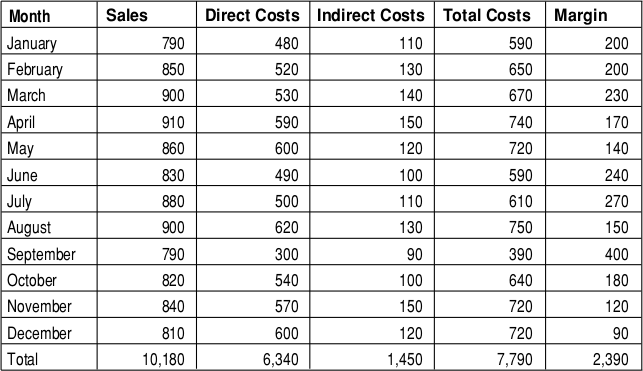
\includegraphics[scale=0.4]{cube_1}
\end{center}
}
\end{frame}


\fbckg{white}
\begin{frame}
\misc
{
Individualmente, \textit{sales}, \textit{costs}, y \textit{margin} representan \textbf{métricas}.

Si alguien pregunta, "¿Qué estás midiendo?".

Le respondemos, "ventas, costos y márgenes".

Los meses representan la organización de los datos.

Ante la pregunta, "¿De dónde consigue sus datos?", o "¿con qué frecuencia está haciendo mediciones?".

Responderíamos, "Estamos siguiendo las ventas mensuales."
\newline


Entonces, utilizando los conceptos dados en la charla \textit{Data Warehouse}, tenemos un \textbf{hecho}, las \textit{variables},
y una \textbf{dimensión}, el \textit{tiempo}.
}
\end{frame}

\fbckg{white}
\begin{frame}
\misc
{
¿Qué sucede cuando añadimos una segunda dimensión llamada \textit{products} (productos)?.
Tenemos un cubo.

\begin{center}
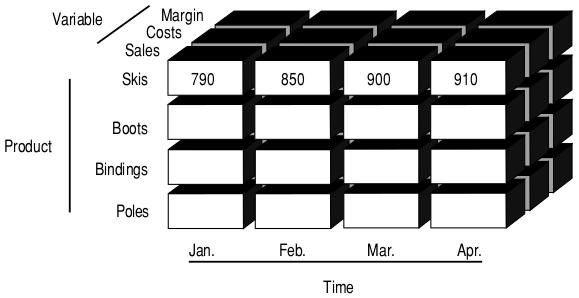
\includegraphics[scale=0.4]{cube_2}
\end{center}
}
\end{frame}


\end{document}
